\documentclass{IEEEtran}
\usepackage{graphicx}
\usepackage{hyperref}

\graphicspath{ {./images/} }

\title{Realtime Food/Non-Food Classification}
\author{Jaime Garcia Diaz [jaimeg4@illinois.edu), Faizan Khan (fkhan71@illinois.edu)}
\date{2021}


\begin{document}

\begin{titlepage}
\maketitle
\end{titlepage}


\begin{abstract}

\end{abstract}


I. INTRODUCTION\\

There's a continuous growing interest in eating healthier that has made available a lot of digital content that provides nutrition facts about the food we eat. At the same time the field of image recognition and data classification has caught the attention of a great number of data scientist enthusiasts and there are multiple papers and projects that have done work on the subject.

After going through the open data on AWS we have chosen to work with the Food-101 database, which has been cited a couple of times in multiple interesting papers that will help to get pieces of the project. However, the part that the papers do not cover as much, is about making the Food/Non-Food classification in real time.\\


II. MODULES\\

The intention of the project is to implement the following modules:\\

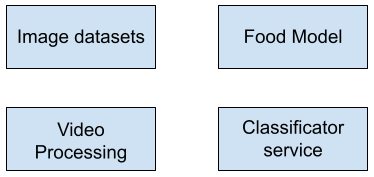
\includegraphics[scale=0.5]{modules}\\

\begin{itemize}
\item \textbf{Image dataset}.
Use a couple of the public datasets and complement them with images from Instagram. 

\item \textbf{Food Model}.
Train a model and so that it could classify images.

\item \textbf{Video Processing}.
Process a video stream into frames, such that the frames could be classified.

\item \textbf{Classification service}.
Setup a service that uses the previous modules and classifies a video feed in real time.\\
\end{itemize}

Below are the pipeline details for our project:\\

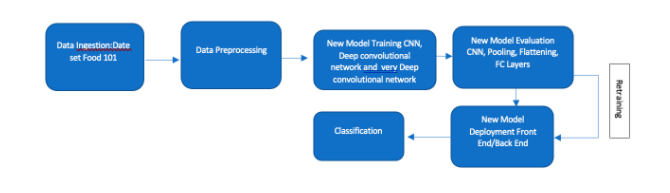
\includegraphics[scale=0.4]{pipeline}\\

III. EXPERIMENTAL SETUP\\

We will be using the AWS resources EMR, DynamoDb and EC2 instances. Project will be done solely using the Python Language and will use Pytorch for deep learning modules. TensorFlow could also be used if needed for more effective visualizations.\\


IV. FUTURE WORK\\

As potential future work, the real time classification could be enhanced by detecting the type of food (ie. pizza or salad, etc.) and while it might be hard to show the actual nutrition facts, at least it should be feasible to display a generic reference for the type of food in the feed.\\


V. REFERENCES\\
\begin{itemize}

\item \href{https://www.semanticscholar.org/paper/An-Efficient-Food-Image-Classification-By-Inception-Burkapalli-Patil/93901843674a8729d2ec6d4b2ac8b1a27b3e0ec6}{An Efficient Food Image Classification By Inception- V3 Based Cnns}

\item \href{https://www.semanticscholar.org/paper/Highly-Accurate-Food%2FNon-Food-Image-Classification-Kagaya-Aizawa/ac72cd1644da89315c44bd2bf320bec7397227a3}{Highly Accurate Food/Non-Food Image Classification Based on a Deep Convolutional Neural Network}

\item \href{https://www.semanticscholar.org/paper/Food-Image-Recognition-Using-Very-Deep-Networks-Hassannejad-Matrella/b69170c11e1808511cc61aa6413ac5f8a6e4d501}{Food Image Recognition Using Very Deep Convolutional Networks}

\item \href{https://www.semanticscholar.org/paper/FACIAL-RECOGNITION-SYSTEM-USING-IMAGE-PROCESSING-ashish-Bimbisara/73dac5236f6a77f45798fa50e2da2effc63a0053}{Facial Recognition System Using Image Processing}

\end{itemize}

\end{document}